\documentclass[journal,twoside,web]{ieeecolor}
\usepackage{tmi}
\usepackage{amsmath,amssymb,amsfonts}
\usepackage{algorithmic}
\usepackage{graphicx}
\graphicspath{{images}}
\usepackage{textcomp}
\def\BibTeX{{\rm B\kern-.05em{\sc i\kern-.025em b}\kern-.08em
    T\kern-.1667em\lower.7ex\hbox{E}\kern-.125emX}}
\markboth{\journalname, VOL. XX, NO. XX, XXXX 2020}
{Author \MakeLowercase{\textit{et al.}}: Preparation of Papers for IEEE TRANSACTIONS ON MEDICAL IMAGING}

\begin{document}
\title{Verarbeitung von Gesichtsaufnahmen zur Genderklassifikation als Anwendung neuronaler Netze}
\author{Niklas Herrhofer, Celine Schneider, Andreas Braig
\thanks{Diese Arbeit wurde im Rahmen des Kurses TEL22AT1 erstellt.}
\thanks{Diese Arbeit wurde am 02.03.2025 eingereicht.}  
\thanks{Die Autoren sind Studierende an der Dualen Hochschule Baden-Württemberg Mannheim.}}

\maketitle

\begin{abstract}
    Brauchen wir echt ein Abstract? 
\end{abstract}


\begin{IEEEkeywords}
    Neuronales Netz, Bildsegmentierung, Convolutional Neural Network, 
\end{IEEEkeywords}

\section{Problemstellung und Ziel dieser Arbeit}
\label{sec:introduction}
\IEEEPARstart{D}{iese} Arbeit befasst sich Mit der Verarbeitung und Klassifikation einzelner Datenpunkte in einem Datensatz.
Die hierbei verwendeten Daten sind Gesichtsaufnahmen verschiedener Personen verschiedenen Alters. 

Die erste Teilaufgabe besteht in der Segmentierung und Verarbeitung dieses bereitgestellten Datensatzes, um die Gesichtselemente einheitlich im Bild zu positionieren. 
Augen und Mund sollen hierbei immer ein gleichschenkliges Dreieck an einer festen Position im Bild bilden. 

Die zweite Teilaufgabe befasst sich mit dem Klassifikationsproblem. 
Der verarbeitete Datensatz wird in ein Convolutional Neural Network geladen und das Geschlecht der abgebildeten Person klassifiziert. 
Hierbei soll das Netz eine binäre Klassifikation zwischen Männlich (0) und Weiblich (1) durchführen.

Für die Lösung dieser Aufgabe wurde die Programmiersprache Python mit den wesentlichen Bibliotheken "OpenCV", "numpy" und "Pytorch" verwendet. 

\section{Stand der Technik}
In diesem Kapitel wird der aktuelle Stand der Technik zur Bildsegmentierung und Klassifizierung Diskutiert.

\subsection{Python}


\subsection{Klassifikationsprobleme}


\begin{figure}[!t]
    \centerline{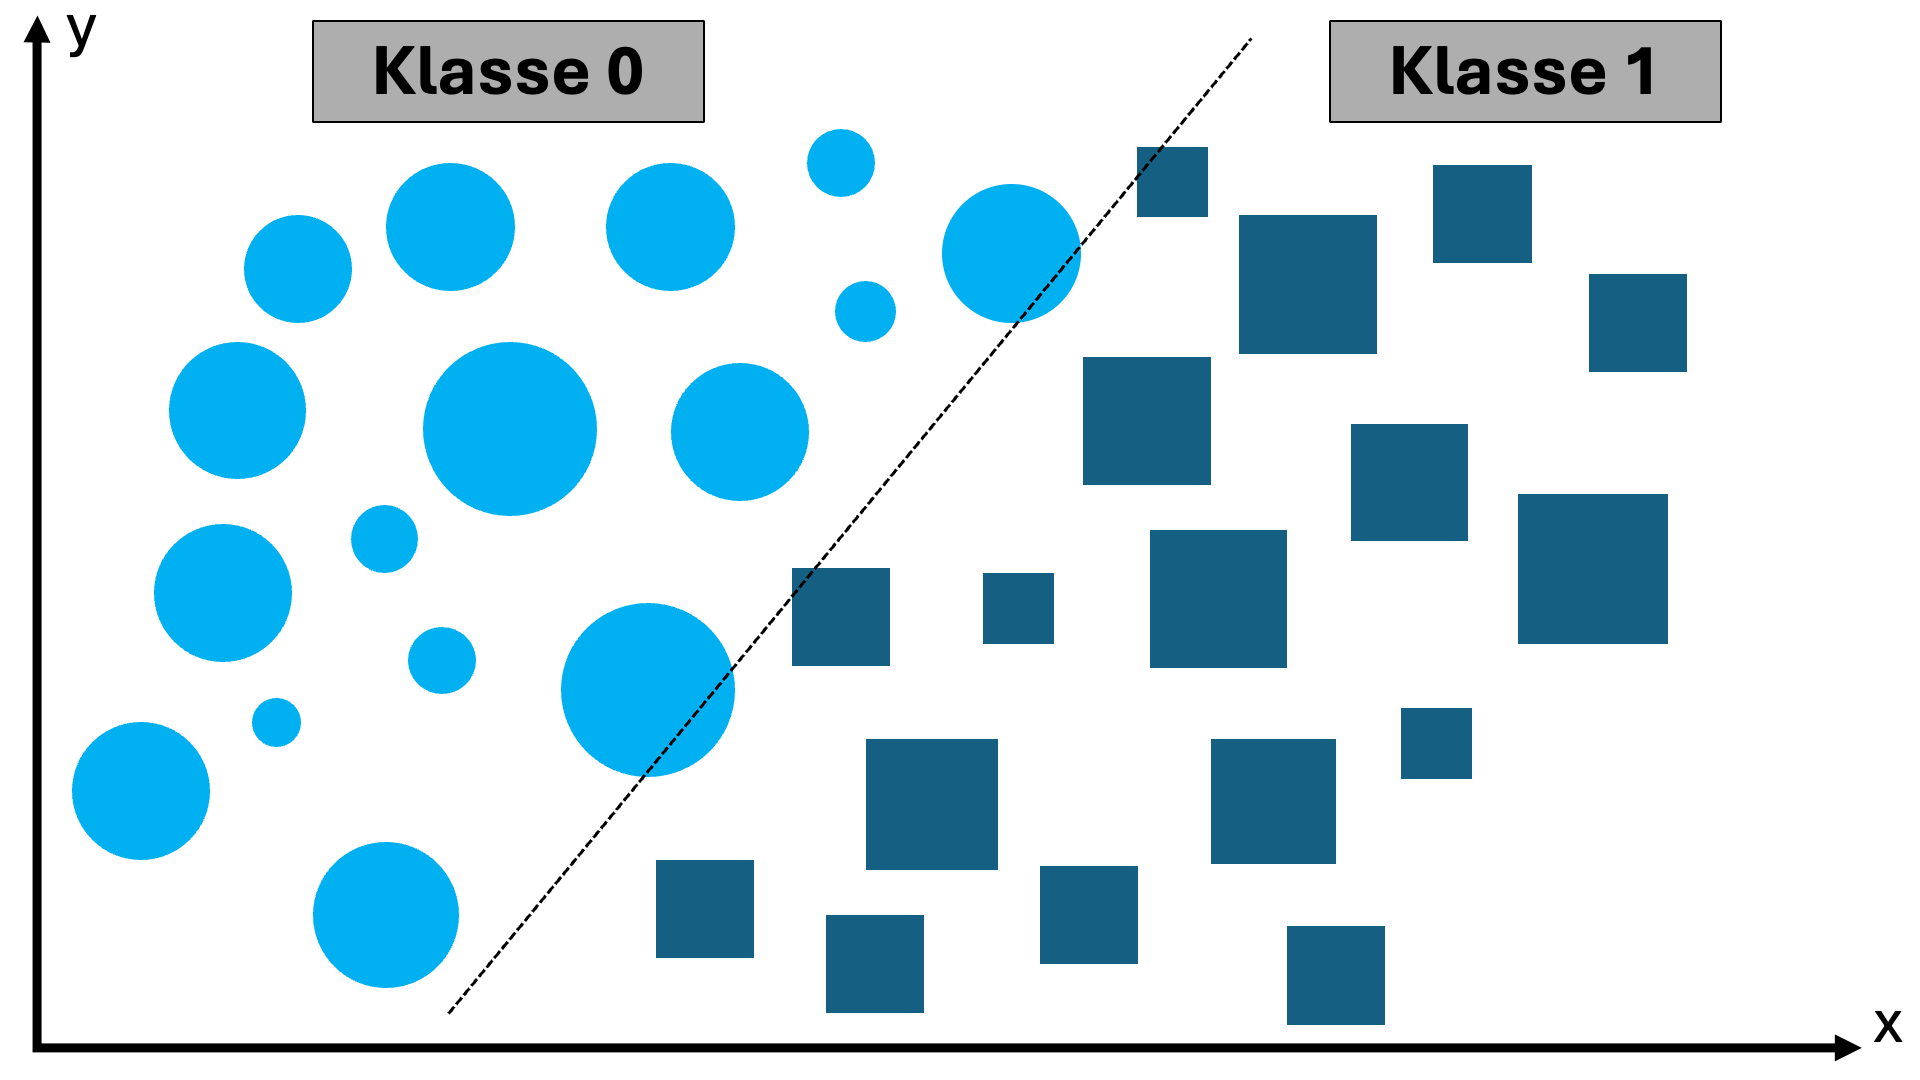
\includegraphics[width=\columnwidth]{Andi/binaere_klassifikation.png}}
    \caption{Magnetization as a function of applied field.
    It is good practice to explain the significance of the figure in the caption.}
    \label{fig:binaere_klassifikation}
\end{figure}



\section{Der Datensatz}
In diesem Kapitel wird der verwendete Datensatz vorgestellt. Es soll nachvollziehbar sein welche Herausforderungen bei der Arbeit mit diesen Daten auftreten. 


\begin{figure}[!t]
\centerline{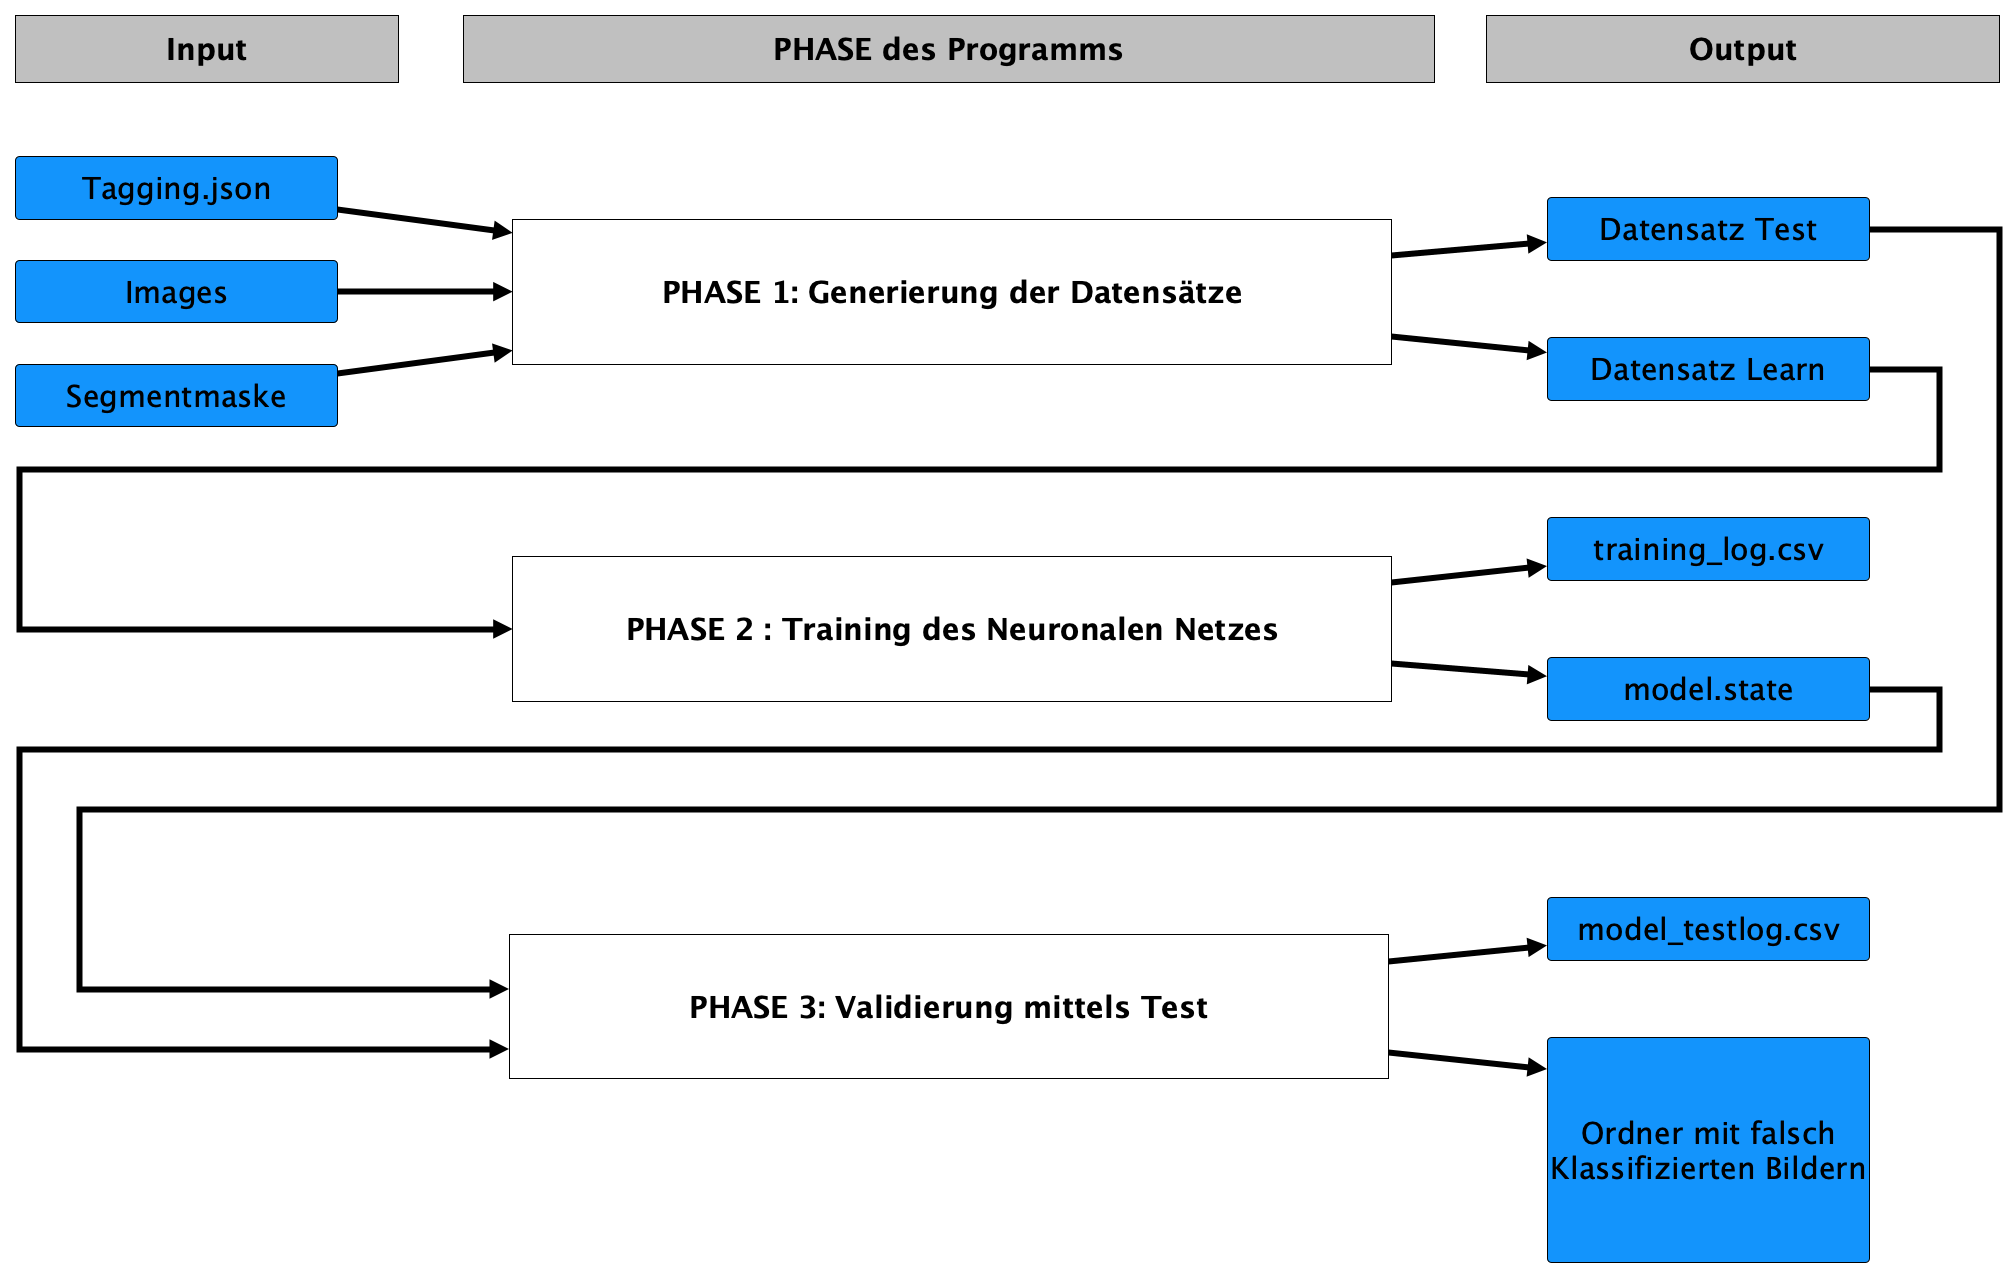
\includegraphics[width=\columnwidth]{Architektur.png}}
\caption{Darstellung der Programmarchitektur in Form eines Blockschaltbildes}
\label{fig:architecture}
\end{figure}




\begin{figure}[!t]
    \centerline{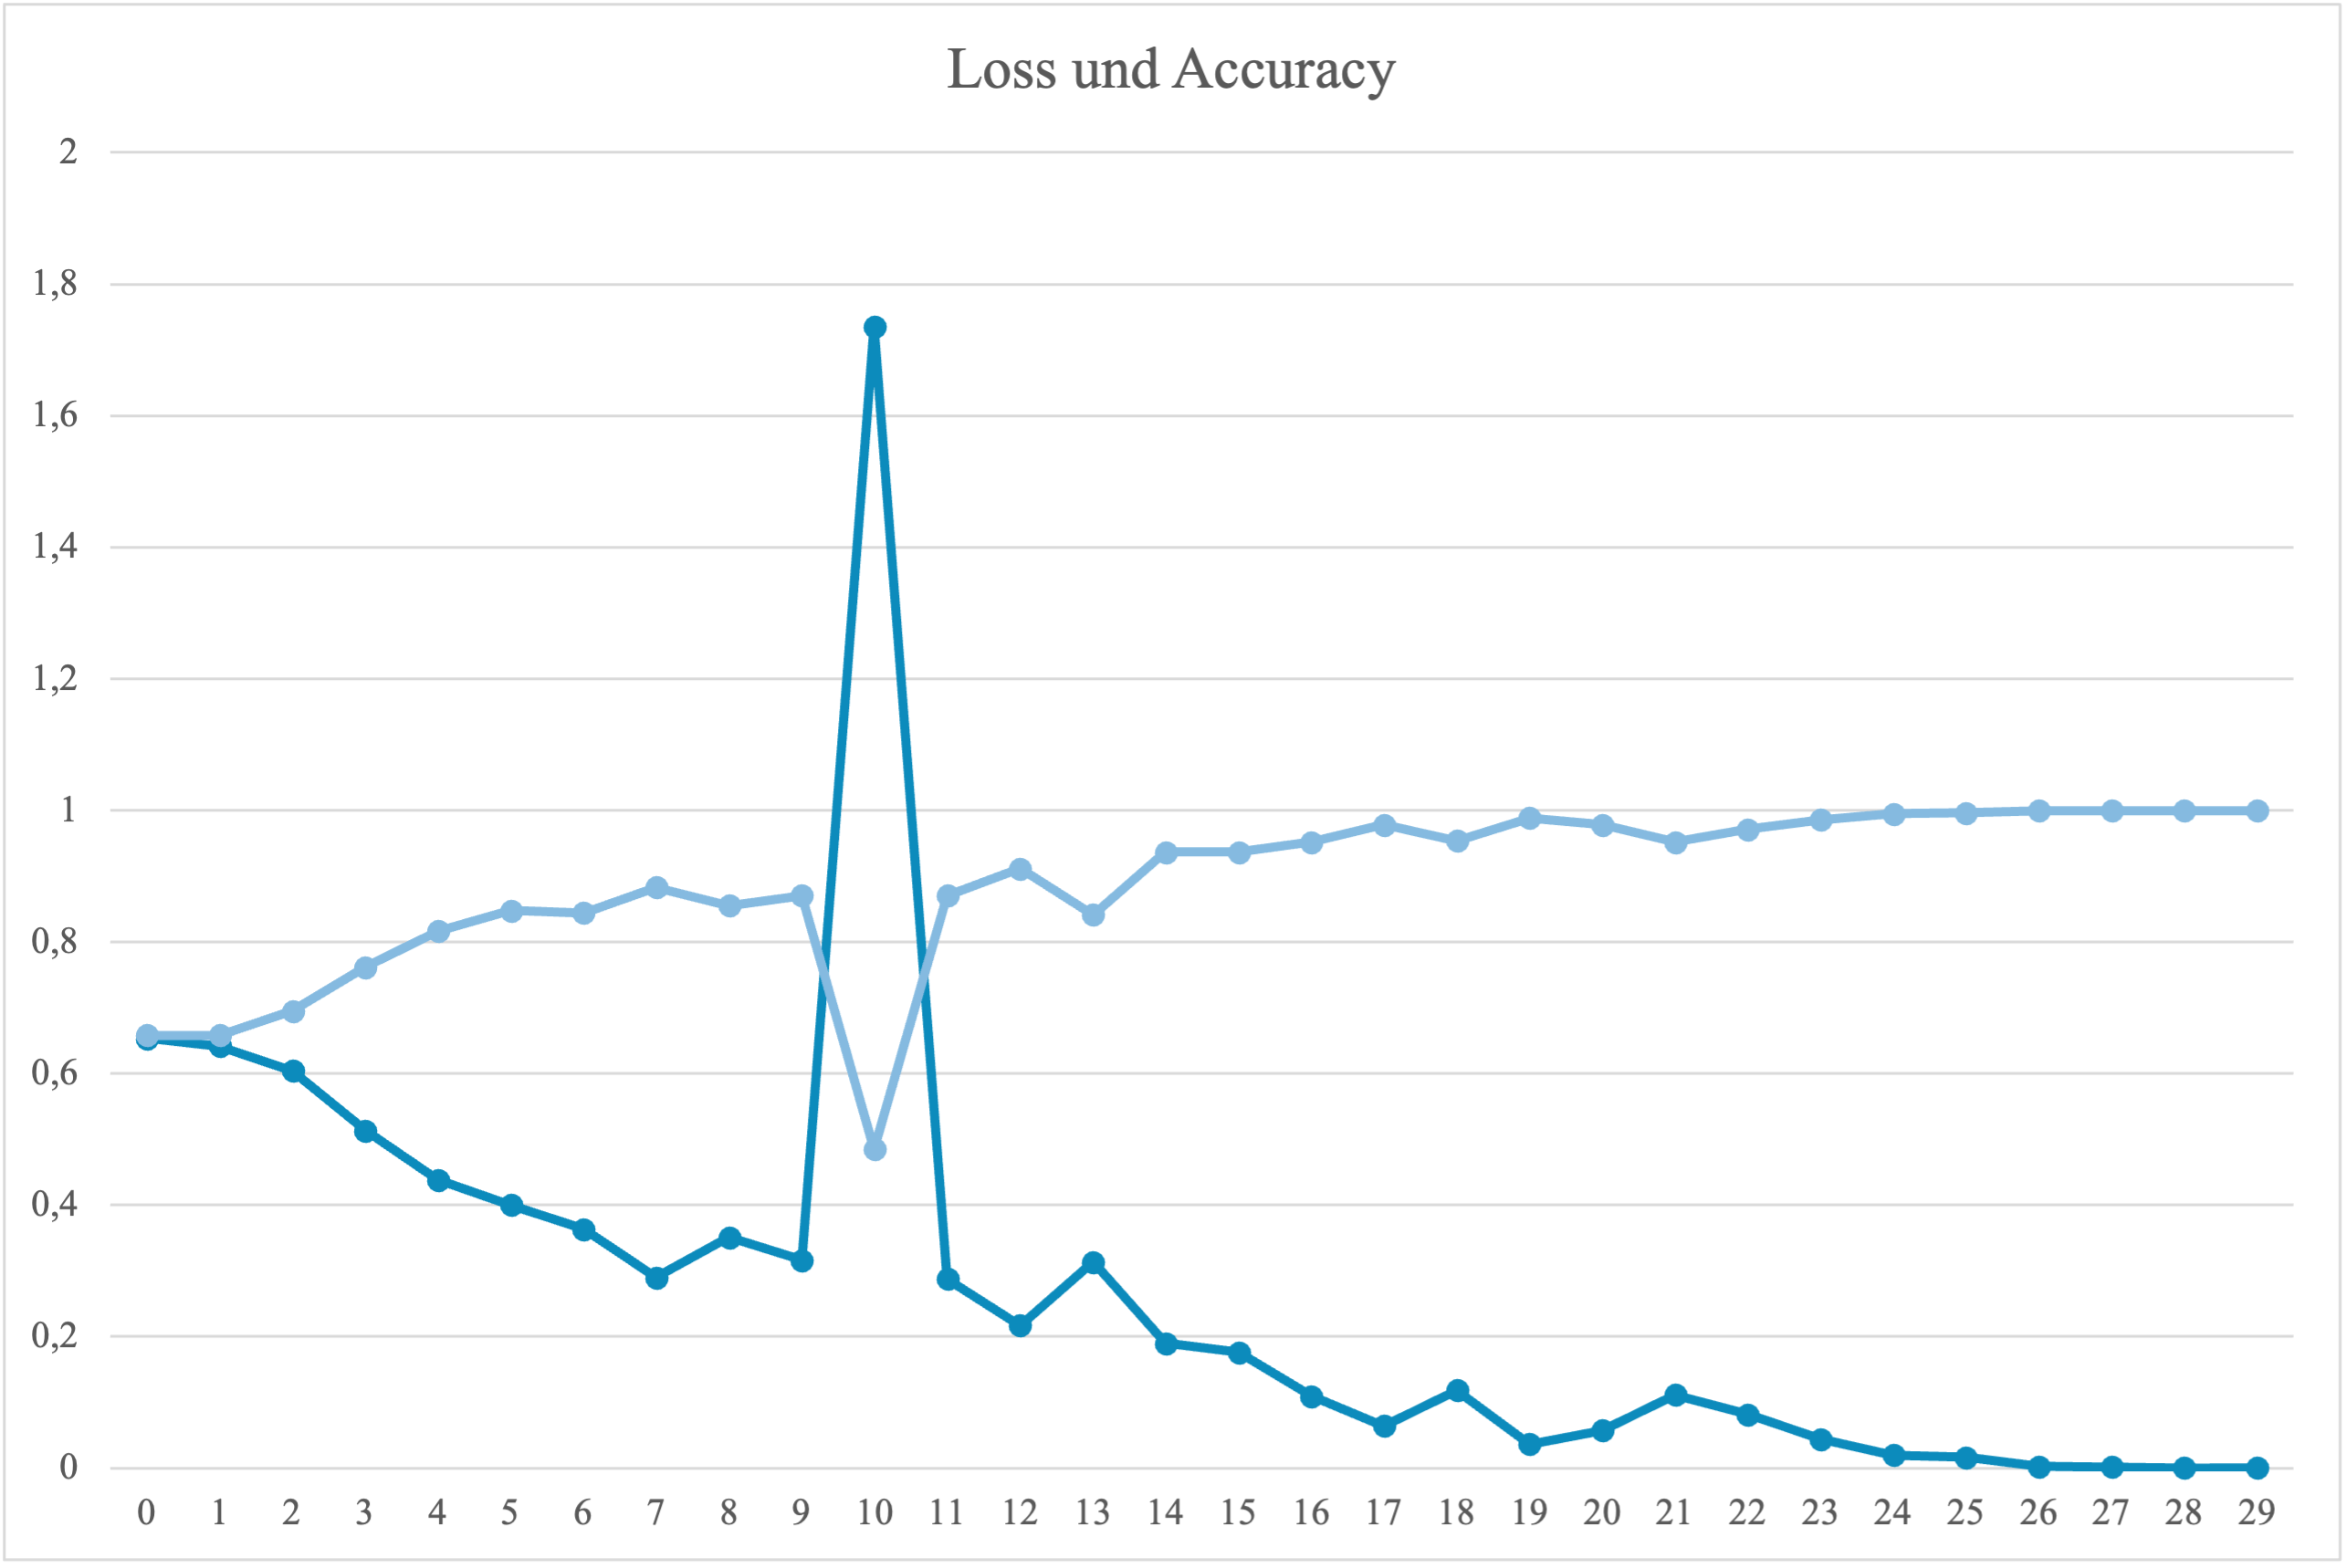
\includegraphics[width=\columnwidth]{Andi/Loss_Acc_Gewinner.png}}
    \caption{Trainingslog des CNN Modells, welches im Test die besten Ergebnisse Erzielt}
    \label{fig:winner}
\end{figure}





\section{Conclusion}


\appendices

\section*{Appendix and the Use of Supplemental Files}


\section*{Acknowledgment}


\end{document}
